\subsection{Effect of the Leak on a Trained Model}
\label{sec:leakmodel}
The persistence numbers above show the leak in the data. To measure its effect on a trained forecaster, we trained the previous model (S2S) and the final model (DS2S) on Starlink DL twice, once with the interpolated inputs of the previous pipeline and once with the causal inputs of this report, with three seeds each (script \texttt{run\_leak.sh}, analysis \texttt{fr\_leak.py}). The models trained on interpolated inputs were tested on both versions of the test inputs. The targets are the same measured series in all cases.

\begin{figure}[H]
  \centering
  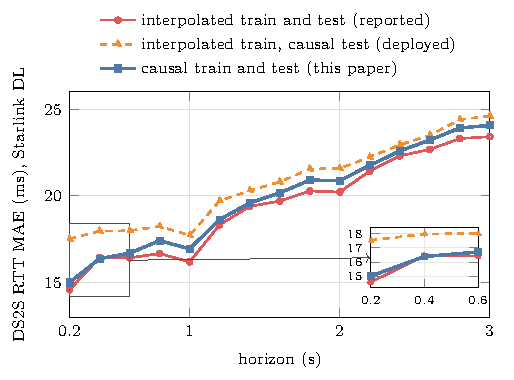
\includegraphics{figs_pdf/fr_leak.pdf}
  \caption{Effect of the interpolation leak on a trained forecaster (DS2S, Starlink DL, mean of three seeds). Trained and tested on interpolated inputs, the model reports a lower error than it reaches when it is deployed on the causal inputs available online. Inset: the first 0.6\,s.}
  \label{fig:leak}
\end{figure}

Fig.~\ref{fig:leak} shows the result. Trained and tested on interpolated inputs, DS2S reports a 0.2\,s RTT MAE of \LeakDSAhOne\,ms. On causal inputs, which are all that a deployed forecaster sees, the same model reaches \LeakDSBhOne\,ms, \LeakOptDSMAEhOne\% worse (RMSE: \LeakOptDSRMSEhOne\%). The model trained on causal inputs reaches \LeakDSChOne\,ms. Causal training therefore also gives the better deployed model. The gap shrinks with the horizon (\LeakOptDSMAEavg\% averaged over 0.2 to 3\,s) and is smaller for S2S (\LeakOptSSMAEhOne\% at 0.2\,s), whose decoder does not start from the last observation. The leak inflates exactly the short-horizon accuracy that a packet scheduler relies on most. The Starlink numbers of the previous report are optimistic for this reason, and every result in this report uses causal inputs.
